\documentclass{beamer}
\usetheme{Frankfurt}

\usepackage{listings}

\newcommand{\todo}[1]{\alert{TODO #1}}

\title{Intrusion Detection}
\subtitle{Lecture 8 \\ Computer Security DD2395}
\author[R. Guanciale]{
  Roberto Guanciale\\
  robertog@kth.se
}
\date{2013-10-03}
\begin{document}

\begin{frame}[plain]
  \titlepage
\end{frame}

\begin{frame}{Computer Security}
  \begin{itemize}
    \item Prevention 
    \item Detection 
    \item Response/Recovery
  \end{itemize}
\end{frame}

\begin{frame}{Intruders}
  \begin{itemize}
  \item significant issue hostile/unwanted trespass 
    \begin{itemize}
    \item from benign to serious 
    \end{itemize}
  \item user trespass 
    \begin{itemize}
    \item unauthorized logon, privilege abuse 
    \end{itemize}
  \item software trespass 
      \begin{itemize}
      \item virus, worm, or trojan horse 
    \end{itemize}
  \item classes of intruders: 
      \begin{itemize}
      \item masquerader, misfeasor, clandestine user
    \end{itemize}
  \end{itemize}
\end{frame}

\begin{frame}{Examples of Intrusion}
  \begin{itemize}
  \item remote root compromise 
  \item web server defacement 
  \item guessing / cracking passwords 
  \item copying viewing sensitive data / databases 
  \item running a packet sniffer 
  \item impersonating a user to reset password 
  \item using an unattended workstation 
  \end{itemize}
\end{frame}

\begin{frame}{Security Intrusion \& Detection}
  \begin{itemize}
  \item Security Intrusion 
    \begin{quote}
a security event, or combination of multiple security 
events, that constitutes a security incident in which an 
intruder gains, or attempts to gain, access to a system 
(or system resource) without having authorization to do 
so. 
    \end{quote}
  \item Intrusion Detection
    
    \begin{quote}
a security service that monitors and analyzes system 
events for the purpose of finding, and providing realtime or near real-time warning of attempts to access 
system resources in an unauthorized manner.
    \end{quote}
  \end{itemize}
\end{frame}

\begin{frame}{Incident}
   \begin{center}
    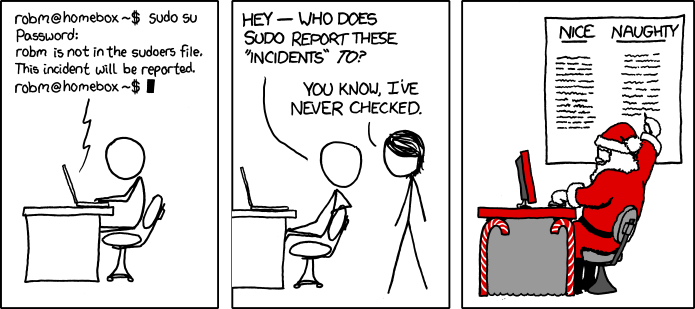
\includegraphics[width=1\linewidth]{incident}
  \end{center}
\end{frame}


\begin{frame}{Hackers}
  \begin{itemize}
  \item Often motivated by thrill of access and status 
    \begin{itemize}
    \item hacking community a strong meritocracy 
    \item status is determined by level of competence 
    \end{itemize}
  \item benign intruders might be tolerable 
    \begin{itemize}
    \item do consume resources and may slow performance 
    \item can't know in advance whether benign or malign 
    \end{itemize}
  \item IDS / IPS / VPNs can help counter 
  \item awareness led to establishment of CERTs 
    \begin{itemize}
    \item collect / disseminate vulnerability info / responses 
    \end{itemize}
  \end{itemize}
\end{frame}

\begin{frame}{Hacker Behavior Example}
  \begin{itemize}
  \item select target using IP lookup tools 
  \item map network for accessible services 
  \item identify potentially vulnerable services 
  \item brute force (guess) passwords
  \item install remote administration tool 
  \item wait for admin to log on and capture password
  \item use password to access remainder of network
  \end{itemize}
\end{frame}

\begin{frame}{Criminal Enterprise}
  \begin{itemize}
  \item \alert{organized} groups of hackers now a threat
    \begin{itemize}
    \item corporation / government / loosely affiliated gangs
    \item common target credit cards on e-commerce server
    \end{itemize}
  \item criminal hackers usually have specific targets
  \item once penetrated act quickly and get out
  \item IDS / IPS help but less effective 
  \item sensitive data needs strong protection
  \end{itemize}
\end{frame}

\begin{frame}{Criminal Enterprise Behavior}
  \begin{itemize}
  \item act quickly and precisely to make their activities 
    harder to detect
  \item exploit perimeter via vulnerable ports
  \item use trojan horses (hidden software) to leave 
    back doors for re-entry
  \item use sniffers to capture passwords
  \item do not stick around until noticed
  \item make few or no mistakes. 
  \end{itemize}
\end{frame}

\begin{frame}{Insider Attacks}
  \begin{itemize}
  \item among most difficult to detect and prevent 
  \item employees have access \& systems knowledge 
  \item may be motivated by revenge / entitlement 
      \begin{itemize}
      \item when employment terminated 
      \item taking customer data when move to competitor 
      \end{itemize}
  \item IDS / IPS may help but also need: 
      \begin{itemize}
      \item least privilege, monitor logs, strong authentication, 
        termination process to block access \& mirror data 
      \end{itemize}
  \end{itemize}
\end{frame}

\begin{frame}{Insider Behavior Example}
  \begin{itemize}
  \item create network accounts for themselves and their 
    friends
  \item access accounts and applications they wouldn't 
    normally use for their daily jobs
  \item e-mail former and prospective employers
  \item conduct furtive instant-messaging chats
  \item visit web sites that cater to disgruntled 
    employees, such as f'dcompany.com
  \item perform large downloads and file copying
  \item access the network during off hours.
  \end{itemize}
\end{frame}

\begin{frame}{Intrusion Techniques}
  \begin{itemize}
  \item objective to gain access or increase privileges
  \item initial attacks often exploit system or software 
    vulnerabilities to execute code to get backdoor
      \begin{itemize}
      \item e.g. buffer overflow 
      \end{itemize}
  \item or to gain protected information 
      \begin{itemize}
      \item e.g. password guessing or acquisition
      \end{itemize}
  \end{itemize}
\end{frame}


\begin{frame}{Intrusion Detection Systems}
  \begin{itemize}
    \item classify intrusion detection systems (IDSs) as:
      \begin{itemize}
      \item Host-based IDS: monitor single host activity
      \item Network-based IDS: monitor network traffic
      \end{itemize}
    \item logical components:
      \begin{itemize}
      \item sensors - collect data
      \item analyzers - determine if intrusion has occurred
      \item user interface - manage / direct / view IDS
      \end{itemize}
  \end{itemize}
\end{frame}

\begin{frame}{IDS Principles}
  \begin{columns}[c]
    \column{0.5\linewidth}
  \begin{itemize}
  \item assume intruder behavior differs from legitimate 
    users 
    \begin{itemize}
    \item expect overlap as shown 
    \item observe deviations 
      from past history 
    \item problems of: 
      \begin{itemize}
      \item false positives 
      \item false negatives 
      \item must compromise 
      \end{itemize}
    \end{itemize}
  \end{itemize}
  \column{0.5\linewidth}
  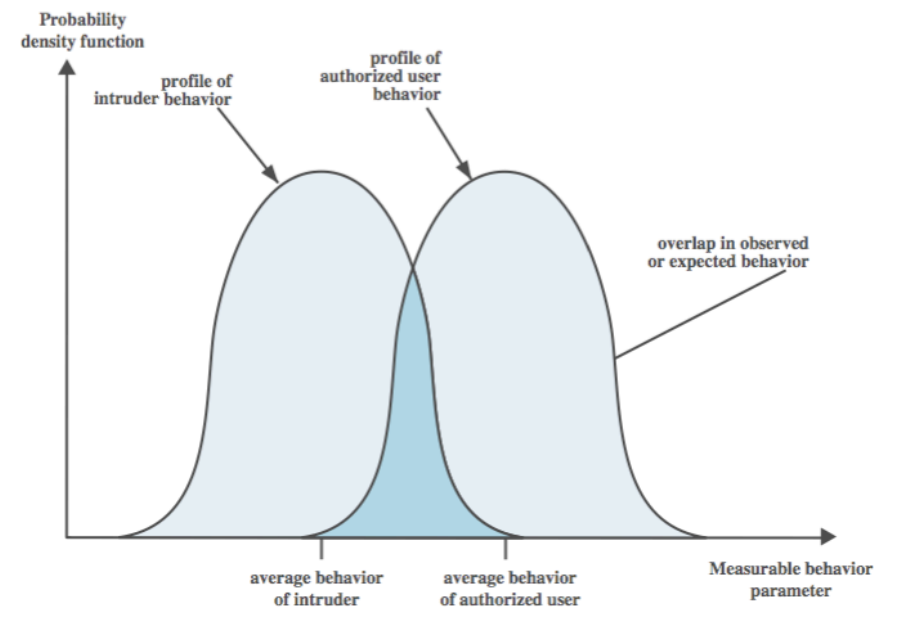
\includegraphics[width=1\linewidth]{falsepositive}
  \end{columns}
\end{frame}

\begin{frame}{IDS Requirements}
  \begin{itemize}
  \item run continually 
  \item be fault tolerant 
  \item resist subversion 
  \item impose a minimal overhead on system 
  \item configured according to system security policies 
  \item adapt to changes in systems and users 
  \item scale to monitor large numbers of systems 
  \item provide graceful degradation of service 
  \item allow dynamic reconfiguration 
  \end{itemize}
\end{frame}

\begin{frame}{Difficult Task}
  \begin{itemize}
  \item Defense has to work all the time, attack only 
    once
  \end{itemize}
  For stories about intrusions, penetration testing, 
see Kevin Mitnick ``The Art of Intrusion''
\end{frame}

\begin{frame}{Host-Based IDS}
  \begin{itemize}
  \item specialized software to monitor system activity to 
    detect suspicious behavior 
    \begin{itemize}
    \item primary purpose is to detect intrusions, log suspicious events, 
      and send alerts 
    \item can detect both external and internal intrusions 
    \end{itemize}
  \item two approaches, often used in combination: 
    \begin{itemize}
    \item anomaly detection - defines normal/expected behavior 
      \begin{itemize}
      \item threshold detection 
      \item profile based 
      \end{itemize}
    \item signature detection - defines proper behavior
    \end{itemize}
  \end{itemize}
\end{frame}


\begin{frame}{Audit Records}
  \begin{itemize}
  \item a fundamental tool for intrusion detection 
  \item two variants: 
    \begin{itemize}
    \item native audit records - provided by O/S 
      \begin{itemize}
      \item always available but may not be optimum 
      \end{itemize}
    \item detection-specific audit records - IDS specific 
      \begin{itemize}
      \item additional overhead but specific to IDS task 
      \item often log individual elementary actions 
      \item e.g. may contain fields for: subject, action, object, 
        exception-condition, resource-usage, time-stamp
      \end{itemize}
    \end{itemize}
  \end{itemize}
\end{frame}

\begin{frame}{Anomaly Detection}
  \begin{itemize}
  \item threshold detection 
    \begin{itemize}
    \item checks excessive event occurrences over time 
    \item alone a crude and ineffective intruder detector 
    \item must determine both thresholds and time intervals 
    \end{itemize}
  \item profile based 
    \begin{itemize}
    \item characterize past behavior of users / groups 
    \item then detect significant deviations 
    \item based on analysis of audit records 
      \begin{itemize}
      \item gather metrics: counter, guage, interval timer, resource utilization
      \item analyze: mean and standard deviation, multivariate, markov 
        process, time series, operational model 
      \end{itemize}
    \end{itemize}
  \end{itemize}
\end{frame}


\begin{frame}{What if \dots}
  \begin{itemize}
  \item You are being hacked while training the 
    system? 
  \item There is a new normal? Difference between 
    abnormal normal and actual attack?
  \end{itemize}
\end{frame}

\begin{frame}{Signature detection}
  \begin{itemize}
  \item observe events on system and applying a set of 
    rules to decide if intruder 
    \begin{itemize}
    \item rule-based penetration identification 
      \begin{itemize}
      \item rules identify known penetrations / weaknesses 
      \item often by analyzing attack scripts from Internet 
      \item supplemented with rules from security experts 
      \end{itemize}
    \end{itemize}
  \end{itemize}
\end{frame}

\begin{frame}{Questions}
  \begin{itemize}
  \item Signature-based IDS: more likely to have 
    \begin{itemize}
    \item[A] false positives or 
    \item[B] false negatives? 
    \end{itemize}
  \item How about anomaly-based IDS? 
    \begin{itemize}
      \item A or B 
    \end{itemize}
  \end{itemize}
\end{frame}

\begin{frame}{Distributed Host-Based IDS}
  
  \begin{center}
    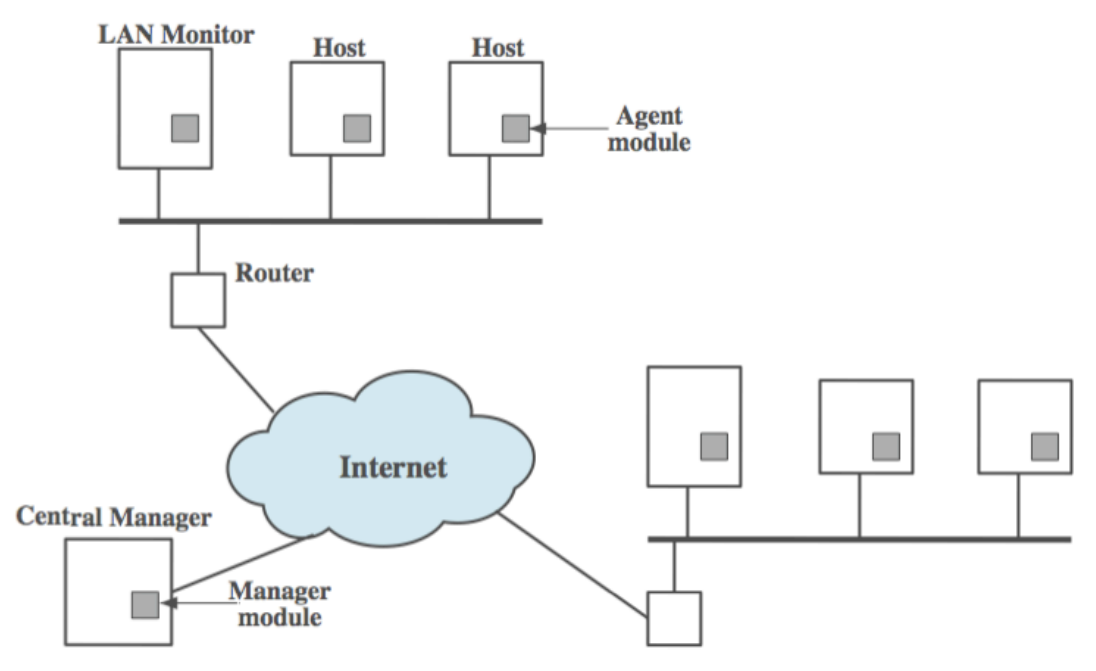
\includegraphics[width=0.9\linewidth]{distributed-host-ids}
  \end{center}
\end{frame}


\begin{frame}{Distributed Host-Based IDS }
  \begin{itemize}
  \item Different audit record formats 
  \item Collection point in network, need to transfer raw 
    data or summaries – confidentiality, integrity 
  \item Centralized vs. decentralized architecture
  \end{itemize}
\end{frame}

\begin{frame}{Network-Based IDS}
  \begin{itemize}
  \item network-based IDS (NIDS) 
    \begin{itemize}
    \item monitor traffic at selected points on a network 
    \item in (near) real time to detect intrusion patterns 
    \item may examine network, transport and/or application 
      level protocol activity directed toward systems 
    \end{itemize}
  \item comprises a number of sensors 
    \begin{itemize}
    \item inline (possibly as part of other net device) 
    \item passive (monitors copy of traffic)
    \end{itemize}
  \end{itemize}
\end{frame}

\begin{frame}{NIDS Sensor Deployment}
   \begin{center}
    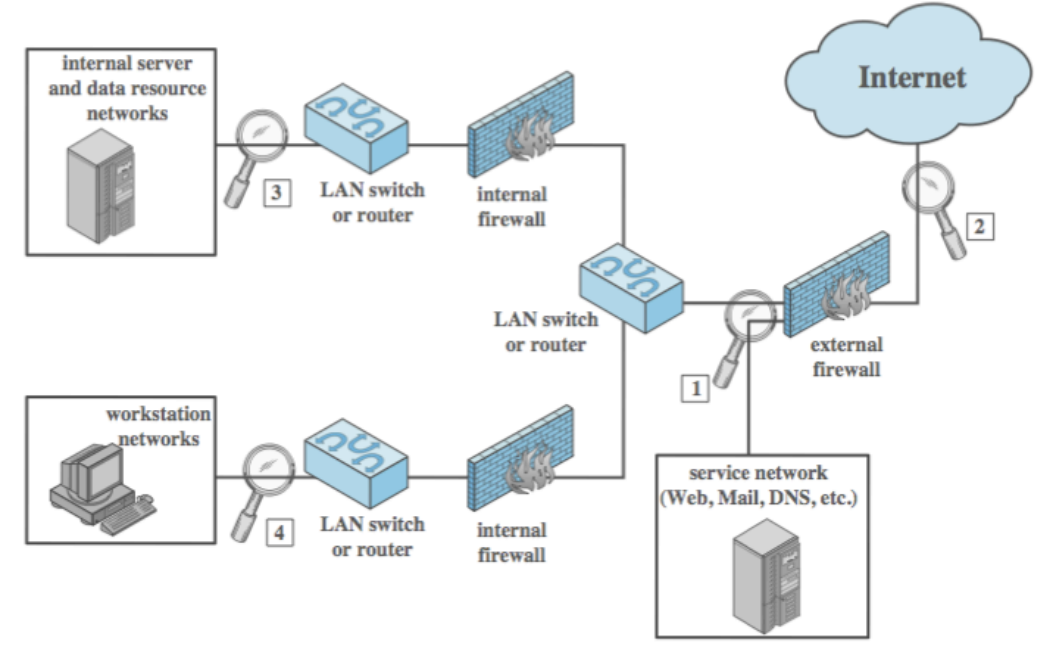
\includegraphics[width=0.9\linewidth]{nids}
  \end{center}
\end{frame}

\begin{frame}{Intrusion Detection Techniques}
  \begin{itemize}
  \item signature detection 
    \begin{itemize}
    \item at application, transport, network layers; unexpected 
      application services, policy violations 
    \end{itemize}
  \item anomaly detection 
    \begin{itemize}
    \item of denial of service attacks, scanning, worms 
    \end{itemize}
  \item when potential violation detected sensor sends an 
    alert and logs information 
    \begin{itemize}
    \item used by analysis module to refine intrusion detection 
      parameters and algorithms 
    \item by security admin to improve protection
    \end{itemize}
  \end{itemize}
\end{frame}

\begin{frame}{Distributed Adaptive Intrusion Detection}
   \begin{center}
    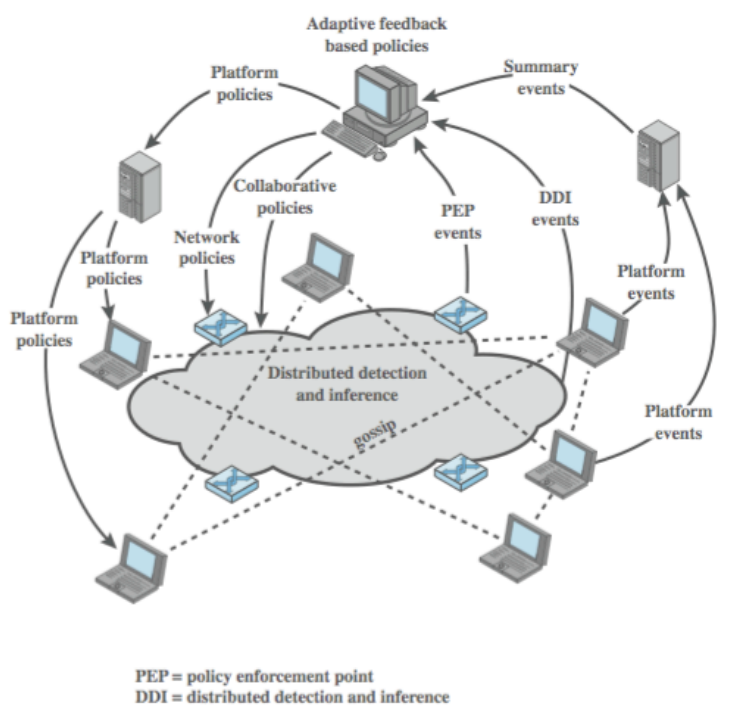
\includegraphics[width=0.6\linewidth]{daids}
  \end{center}
\end{frame}

\begin{frame}{Intrusion Detection Exchange Format}
   \begin{center}
    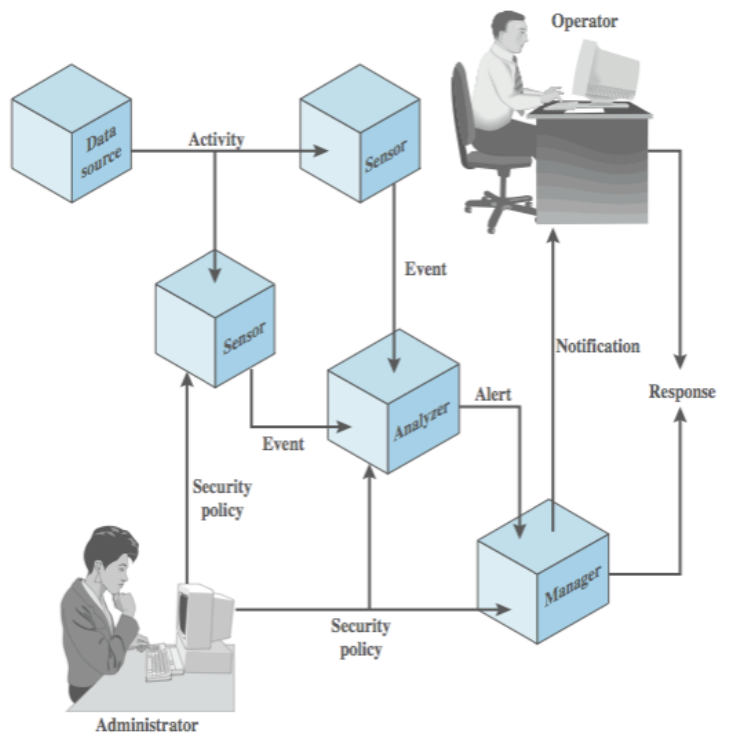
\includegraphics[width=0.6\linewidth]{ids-format}
  \end{center}
\end{frame}

\begin{frame}{Honeypots}
  \begin{itemize}
  \item are decoy systems 
    \begin{itemize}
    \item filled with fabricated info 
    \item instrumented with monitors / event loggers 
    \item divert and hold attacker to collect activity info 
    \item without exposing production systems 
    \end{itemize}
  \item initially were single systems 
  \item more recently are/emulate entire networks
  \end{itemize}
\end{frame}

\begin{frame}{Honeypot Deployment}
   \begin{center}
    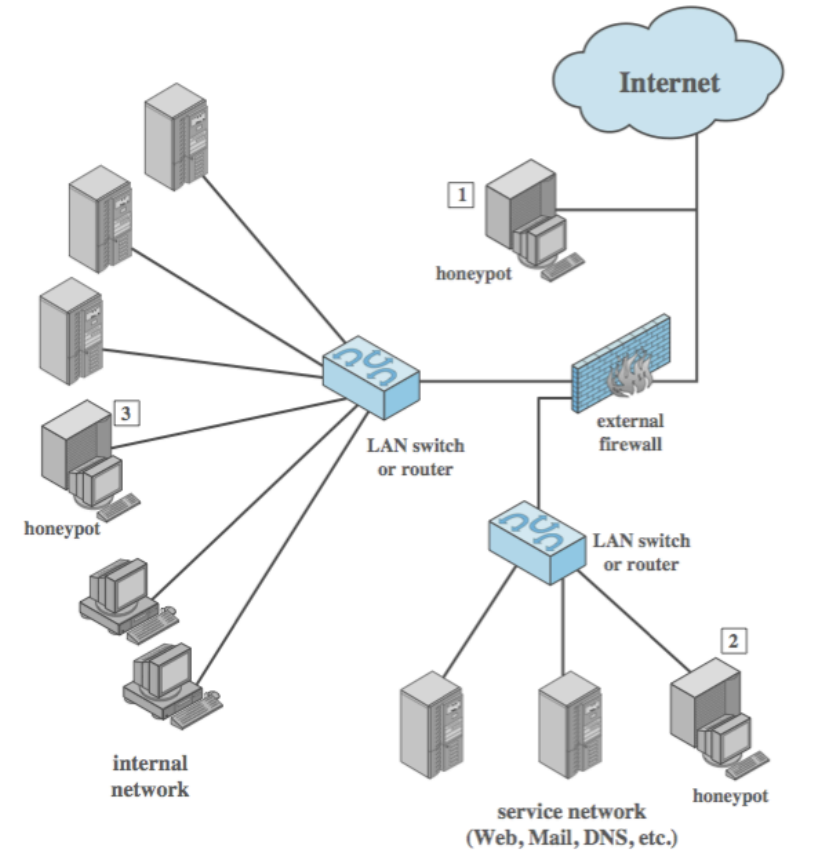
\includegraphics[width=0.6\linewidth]{honeypot}
  \end{center}
\end{frame}

\begin{frame}{Risks of Honeypots?}
\end{frame}

\begin{frame}{SNORT}
  \begin{itemize}
  \item lightweight IDS 
    \begin{itemize}
    \item real-time packet capture and rule analysis 
    \item passive or inline
    \end{itemize}
  \end{itemize}
   \begin{center}
    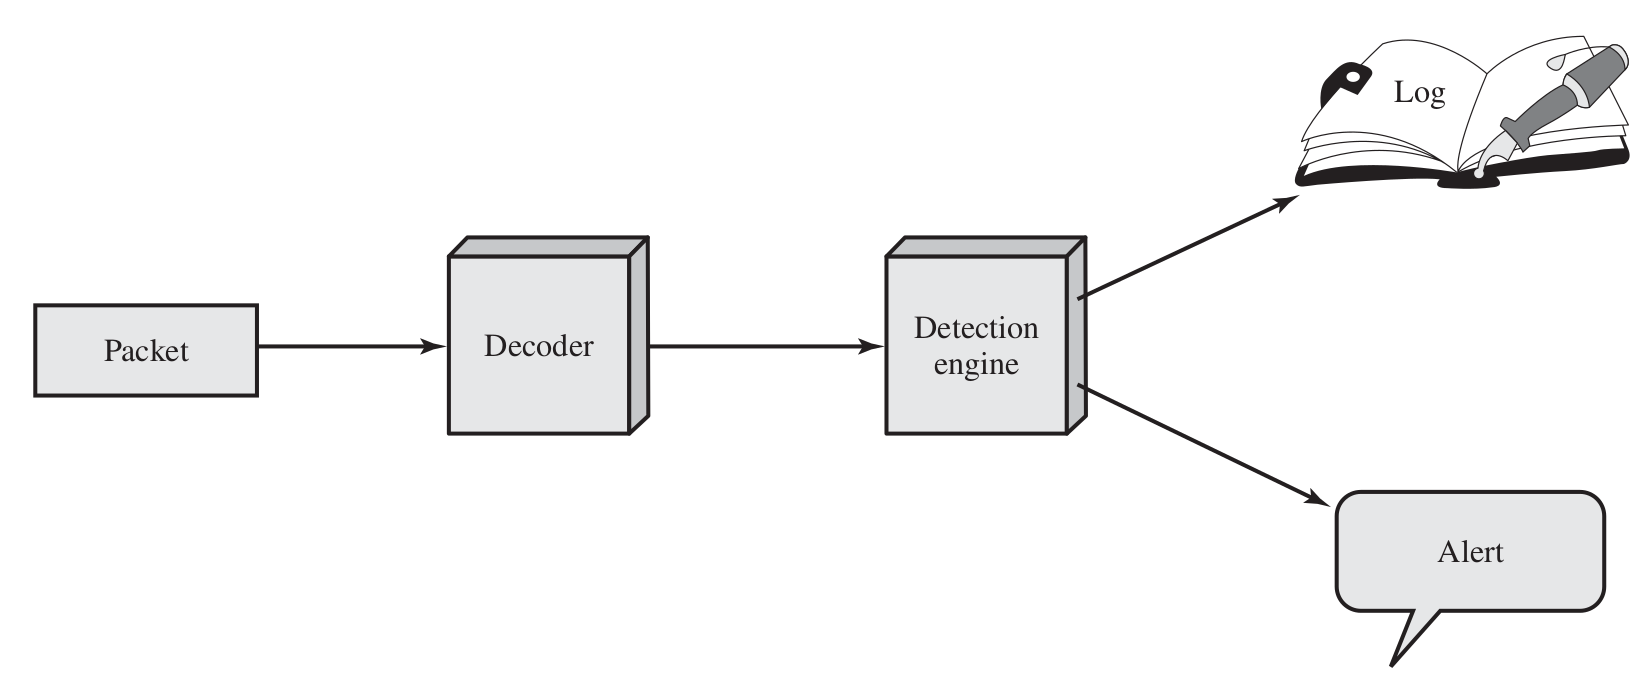
\includegraphics[width=1\linewidth]{snort}
  \end{center}
\end{frame}

\begin{frame}[fragile]{SNORT Rules}
  \begin{itemize}
  \item use a simple, flexible rule definition language 
  \item with fixed header and zero or more options 
  \item header includes: action, protocol, source IP, source 
    port, direction, dest IP, dest port 
  \item many options 
  \item example rule to detect TCP SYN-FIN attack:   
    \begin{verbatim}
Alert tcp $EXTERNAL_NET any -> $HOME_NET any \
(msg: "SCAN SYN FIN"; flags: SF, 12; \
reference: arachnids, 198; \
classtype: attempted-recon;)
    \end{verbatim}
  \end{itemize}
\end{frame}

\begin{frame}{Limitations of Intrusion Detection}
See Ross Anderson's book: 
  \begin{itemize}
  \item Detecting viruses as hard as the halting problem 
  \item 2 types of intrusions: error-causing or not 
  \item Response can lead to DoS
  \item False alarms, users/attackers get around them 
  \item Rules: discrimination, data protection law: citizens are 
    entitled to know the algorithms used to process their 
    personal data
  \end{itemize}
\end{frame}

\begin{frame}{Limitations of Intrusion Detection}
  \begin{itemize}
  \item NW: Internet is noisy (bugs, out-of-date DNS), leads to 
    false positives 
  \item ``too few attacks'' – base rate fallacy 
  \item Version-specific attacks, constant need for updates 
  \item Due diligence only, lack of updates 
  \item Encrypted traffic hard to analyze 
  \item Trade-offs, as in firewalls, low-level analysis fast but 
    can have fragmentation, higher-level intensive and 
    frequent updates 
  \item Stealthy attacks 
  \end{itemize}
\end{frame}

\begin{frame}{Summary}
  \begin{itemize}
  \item introduced intruders \& intrusion detection 
    \begin{itemize}
    \item hackers, criminals, insiders 
    \end{itemize}
  \item intrusion detection approaches 
    \begin{itemize}
    \item host-based (single and distributed) 
    \item network 
    \item distributed adaptive 
    \item exchange format 
    \end{itemize}
  \item honeypots 
  \item SNORT example 
  \item limitations
  \end{itemize}
\end{frame}




\end{document}




%%% Local Variables: 
%%% mode: latex
%%% TeX-master: t
%%% End: 
